\section*{Sled localization}
    Considering that the rope remains continuously under tension while the robot is moving, then the evolution of the angle $x_4$ of the sled relative to the towing vehicle is described by the \textit{Differential Equation}~\ref{eq:phi}.

    Then we are able to find the trajectory of the sled by calculating the interval containing the angle $x_4$. The idea is to consider that initially $x_4$ belongs to $[-\pi/2; \pi/2]$. Then by applying \textit{Equation}~\ref{eq:phi} on this interval, we end up obtaining a fine interval framing the real angle $x_4$, independently of the initial angle as we can see on the \textsc{Figure}~\ref{fig:integration}.

    \begin{figure}[!htb]
        \centering
        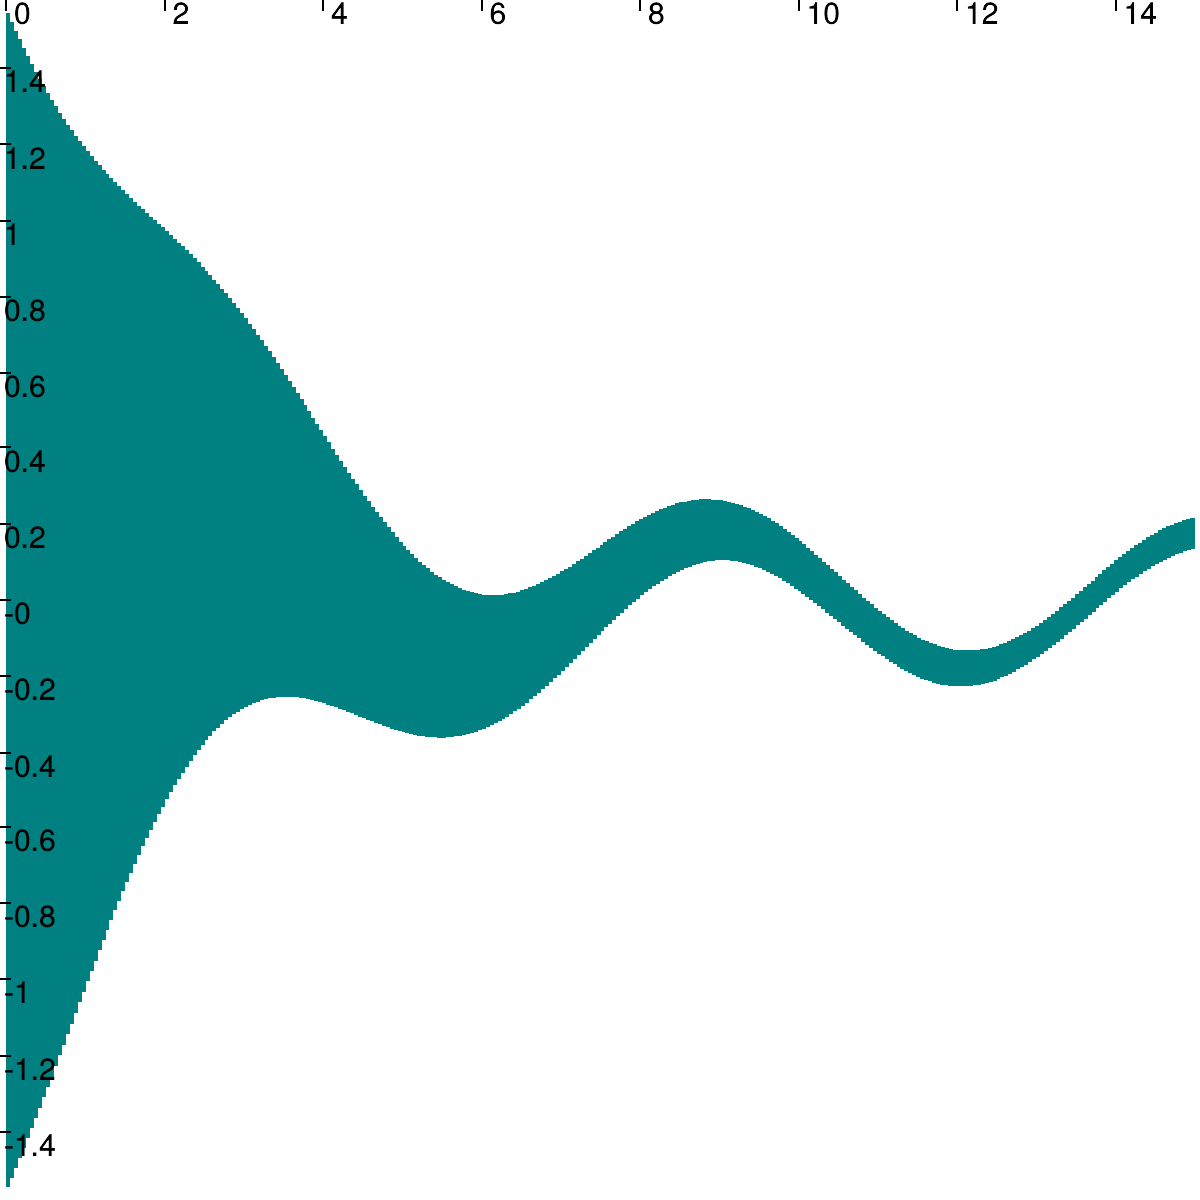
\includegraphics[width=0.35\textwidth]{imgs/integration_example.png}
        \caption{\label{fig:integration} Integration example using intervals}
    \end{figure}

    By having an interval framing the angle $x_4$, we are able to obtain a box containing the sled, knowing the length of the rope.
    This box has the shape of a pie sector. \textit{Equation}~\ref{eq:magnetometer} presents the position of the magnetometer as a function of the state of the system $x_1$, $x_2$ and $x_4$. Here all these variables are intervals. By applying a polar contractor to these intervals, we are able to obtain the intervals containing $x_m$ and $y_m$.

    \begin{equation}\label{eq:magnetometer}
        \left\lbrace
            \begin{aligned}
                x_m &= x_1 - L.cos(x_4) \\
                y_m &= x_2 - L.sin(x_4)
            \end{aligned}
        \right.
    \end{equation}